%%%%%%%%%%%%%%%%%%%%%%%%%%%%%%%%%%%%%%%%%%%%%%%%%%%%%%%%%%%%%%%%%%%%%%%%%%%%%%%%%%
\begin{frame}[fragile]\frametitle{}
\begin{center}
{\Large Operators}
\end{center}
\end{frame}

%%%%%%%%%%%%%%%%%%%%%%%%%%%%%%%%%%%%%%%%%%%%%%%%%%%%%%%%%%%%%%%%%%%%%%%%%%%%%%%%%%%
\begin{frame}[fragile]\frametitle{Operators}
\begin{itemize}
\item The usual unary and binary arithmetic operators: $+,-,*,/,**,<<,>>$, etc.
\item Logical operators: \texttt{and}, \texttt{or}, \texttt{not}.
\item Numerical and string comparison: \texttt{<}, \texttt{>}, \texttt{<=}, \texttt{==}, \texttt{!=}, \ldots
\item Order of operations: PEMDAS: Parentheses, Exponentiation,  Multiplication, Division, Addition and Subtraction.
\item  Operators with the same precedence are evaluated from left to right.
\end{itemize}
\end{frame}

%%%%%%%%%%%%%%%%%%%%%%%%%%%%%%%%%%%%%%%%%%%%%%%%%%%%%%%%%%%%%%%%%%%%%%%%%%%%%%%%%%%
\begin{frame}[fragile] \frametitle{First exercise}
Calculate:
  \begin{center}
    {\Large How much is \href{http://www.pythonchallenge.com}{$2^{38}$} ?}
  \end{center}

\end{frame}

%%%%%%%%%%%%%%%%%%%%%%%%%%%%%%%%%%%%%%%%%%%%%%%%%%%%%%%%%%%%%%%%%%%%%%%%%%%%%%%%%%%
\begin{frame}[fragile]\frametitle{Operators}
  Some operators are defined for non-numeric types:
\begin{lstlisting}
>>> "U" + 'ZH'
'UZH'
\end{lstlisting}

  
  Some support operands of mixed type:
\begin{lstlisting}
>>> "a" * 2
'aa'
>>> 2 * "a"
'aa'
\end{lstlisting}

  
  Some do not:
\begin{lstlisting}[basicstyle=\footnotesize\ttfamily]
>>> "aaa" / 3
Traceback (most recent call last):
  File "<stdin>", line 1, in <module>
TypeError: unsupported operand type(s) for /: 'str' and 'int'
\end{lstlisting}
\end{frame}

%%%%%%%%%%%%%%%%%%%%%%%%%%%%%%%%%%%%%%%%%%%%%%%%%%%%%%%%%%%%%%%%%%%%%%%%%%%%%%%%%%%%
%\begin{frame}[fragile]\frametitle{Area of Triangle}
%Python program to find the largest number among the three input numbers
%\begin{lstlisting}
%s = (a+b+c)/2
%area = sqrt(s(s-a)*(s-b)*(s-c))
%\end{lstlisting}
%
%\begin{lstlisting}
%a = 5
%b = 6
%c = 7
%
%# calculate the semi-perimeter
%s = (a + b + c) / 2
%
%# calculate the area
%area = (s*(s-a)*(s-b)*(s-c)) ** 0.5
%print('The area of the triangle is %0.2f' %area)
%\end{lstlisting}
%\end{frame}


%%%%%%%%%%%%%%%%%%%%%%%%%%%%%%%%%%%%%%%%%%%%%%%%%%%%%%%%%%%%%%%%%%%%%%%%%%%%%%%%%%%
\begin{frame}[fragile]\frametitle{Operators}
There are two kinds of division operators:
\begin{itemize}
\item  "true division" performed by "/"
\item  "floor division" performed by "//"

\end{itemize}

  \begin{lstlisting}
  >>> 10 / 3
3.3333333333333335
>>> 10.0 / 3.0
3.3333333333333335
>>> 10.5 / 3.5
3.0
>>> 

>>> 9 // 3
3
>>> 10 // 3
3
>>> 11 // 3
3
>>> 12 // 3
4
>>> 10.0 // 3
3.0
  \end{lstlisting}

\end{frame}


%%%%%%%%%%%%%%%%%%%%%%%%%%%%%%%%%%%%%%%%%%%%%%%%%%%%%%%%%%%%%%%%%%%%%%%%%%%%%%%%%%%
\begin{frame}[fragile]\frametitle{Operators}

The ``\texttt{\%}'' operator computes the remainder of integer division.
  \begin{lstlisting}
>>> remainder = 7 % 3
>>> print(remainder)
1
  \end{lstlisting}

\end{frame}

% %%%%%%%%%%%%%%%%%%%%%%%%%%%%%%%%%%%%%%%%%%%%%%%%%%%%%%%%%%%%%%%%%%%%%%%%%%%%%%%%%%%
% \begin{frame}[fragile]\frametitle{Operators}
% \begin{itemize}
% \item   Expressions : operations that manipulate values and return something.
% \item  For instance, \texttt{2+2} is an expression
% \item \emph{Not all Python constructs return a value.}  (Assignment, for example, does not.)
% \end{itemize}
% \end{frame}


%%%%%%%%%%%%%%%%%%%%%%%%%%%%%%%%%%%%%%%%%%%%%%%%%%%%%%%%%%%%%%%%%%%%%%%%%%%%%%%%%%%
\begin{frame}[fragile] \frametitle{Operators}
The + operator works with strings, but it is not addition in the mathematical sense. Instead it performs concatenation.
\begin{lstlisting}
>>> first = 10
>>> second = 15
>>> print(first+second)
25
>>> first = '100'
>>> second = '150'
>>> print(first + second)
100150
\end{lstlisting}
\end{frame}

%%%%%%%%%%%%%%%%%%%%%%%%%%%%%%%%%%%%%%%%%%%%%%%%%%%%%%%%%%%%%%%%%%%%%%%%%%%%%%%%%%%
\begin{frame}[fragile] \frametitle{Operators}
Use assignment `\texttt{=}' statement:
\begin{lstlisting}
>>> a = 1
>>> print(a)
1
\end{lstlisting}
Shortcut notations:
  \begin{itemize}
  \item[] \texttt{\emph{a} += \emph{b}} short for \texttt{\emph{a} = \emph{a} + \emph{b}},
  \item[] \texttt{\emph{a} -= \emph{b}} short for \texttt{\emph{a} = \emph{a} - \emph{b}},
  \item[] \texttt{\emph{a} *= \emph{b}} short for \texttt{\emph{a} = \emph{a} * \emph{b}},
   \end{itemize}
\end{frame}

% %%%%%%%%%%%%%%%%%%%%%%%%%%%%%%%%%%%%%%%%%%%%%%%%%%%%%%%%%%%%%%%%%%%%%%%%%%%%%%%%%%%
% \begin{frame}[fragile] \frametitle{Assignment, II}

  % \textbf{Python variables are just ``names'' given to values.}
  
  % Handles \ldots References
  
  % Reference to the string \texttt{'Hello!'} by the \emph{name} \texttt{a}:

% \begin{center}
% 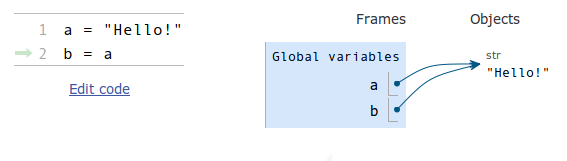
\includegraphics[width=\linewidth,keepaspectratio]{a=b.png}
% \end{center}
  
% The same object can be given many names!
% \end{frame}

%%%%%%%%%%%%%%%%%%%%%%%%%%%%%%%%%%%%%%%%%%%%%%%%%%%%%%%%%%%%%%%%%%%%%%%%%%%%%%%%%%%
\begin{frame}[fragile]  \frametitle{The \texttt{is} operator}

  Allows to test whether two names refer  to the same object:
\begin{lstlisting}
>>> a = 1
>>> b = 1
>>> a is b
True
\end{lstlisting}

\end{frame}

% %%%%%%%%%%%%%%%%%%%%%%%%%%%%%%%%%%%%%%%%%%%%%%%%%%%%%%%%%%%%%%%%%%%%%%%%%%%%%%%%%%%
% \begin{frame}[fragile]\frametitle{Sample Program}
% \begin{itemize}
% \item Upon taking this class, you are recruited in a new hot startup. 
% \item They offer you a decent starting salary (Rs. 50K), a promised 25\% bonus, and an equity package currently worth Rs. 400K, vesting over a period of 4 years.
% \end{itemize}
% \end{frame}


% % %%%%%%%%%%%%%%%%%%%%%%%%%%%%%%%%%%%%%%%%%%%%%%%%%%%%%%%%%%%%%%%%%%%%%%%%%%%%%%%%%%%
% % \begin{frame}[fragile]\frametitle{Sample Program}
% % \begin{itemize}

% % \item You want to examine the true value of this package, so you write the following program:
% % \begin{lstlisting}
% % base_salary = 50000
% % expected_bonus = 0.25
% % equity = 400000
% % years_vesting = 4
% % \end{lstlisting}
% % \item Formula
% % \begin{lstlisting}
% % yearly_value = base_salary + expected_bonus*base_salary + equity/years_vesting
% % print("The yearly value of this offer is", yearly_value)
% % \end{lstlisting}
% % \end{itemize}
% % \end{frame}

%%%%%%%%%%%%%%%%%%%%%%%%%%%%%%%%%%%%%%%%%%%%%%%%%%%%%%%%%%%%%%%%%%%%%%%%%%%%%%%%%%%
\begin{frame}[fragile]\frametitle{Exercise, I}
\begin{itemize}
\item Assume that you go to a restaurant, and you order Rs.50 worth of food. 
\item Then you need to add the Sales Tax (8.875\%) and add a tip (say, 20\%). 
\item Write down the calculation that will print the total cost of the food.
\end{itemize}
\end{frame}
%%%%%%%%%%%%%%%%%%%%%%%%%%%%%%%%%%%%%%%%%%%%%%%%%%%%%%%%%%%%%%%%%%%%%%%%%%%%%%%%%%%
\begin{frame}[fragile]\frametitle{Exercise, II}
\begin{itemize}
\item You have a stock that closed at Rs.550 on Monday, and then closed at Rs.560 on Tuesday.
\item Calculate its daily return: the daily return is defined as the difference in the closing prices, divided by the closing price the day before.
\end{itemize}
\end{frame}

%%%%%%%%%%%%%%%%%%%%%%%%%%%%%%%%%%%%%%%%%%%%%%%%%%%%%%%%%%%%%%%%%%%%%%%%%%%%%%%%%%%
\begin{frame}[fragile]\frametitle{Exercise, III}
\begin{itemize}
\item Write a Python program to solve $(x + y) * (x + y)$
\item Write a Python program to compute the future value of a specified principal amount, rate of interest, and a number of years.  Test Data : amt = 10000, int = 3.5, years = 7.
Expected Output : 12722.79
\item Write a Python program to compute the distance between the points (x1, y1) and (x2, y2).
\end{itemize}
\end{frame}
